\documentclass{assignment}

\usepackage{float}
\usepackage{tikz}
\usepackage{adjustbox}
\usepackage{titlesec}
\usepackage{soul}
\usepackage{csvsimple}

\usepackage{bm}
\usepackage{amsmath,amssymb}

\usepackage{pgfplots}
\usepackage{graphics, epsfig}

\usepackage{graphicx}
\usepackage{subcaption}
\usepackage{matlab-prettifier}
\usepackage{multirow}

\usetikzlibrary{decorations.pathmorphing, decorations.markings}
\usetikzlibrary{positioning}

\usetikzlibrary{calc,patterns,angles,quotes}
\setlength{\parindent}{0pt}

\usetikzlibrary{shapes, arrows}
\tikzstyle{startstop} = [rectangle, rounded corners, minimum width=3cm, minimum height=1cm, text centered, draw=black, fill=red!30]
\tikzstyle{io} = [trapezium, trapezium stretches=true, trapezium left angle=70, trapezium right angle=110, minimum width=4cm, minimum height=1cm, text centered, draw=black, fill=blue!30]
\tikzstyle{process} = [rectangle, minimum width=4cm, minimum height=1cm, text centered, text width=4cm, draw=black, fill=orange!30]
\tikzstyle{decision} = [diamond, minimum width=3cm, minimum height=1cm, text centered, draw=black, fill=green!30]
\tikzstyle{arrow} = [thick,->,>=stealth]

\hypersetup{
pdftitle={Autonomous Vehicles},
pdfsubject={Assignment V},
pdfauthor={Tommaso Bocchietti}
}

\makeglossaries

\begin{document}

\title{Autonomous Vehicles \\ Assignment V: Finite State Machines}
\author{Tommaso Bocchietti 10740309}
\date{A.Y. 2024/25}

\maketitle

\begin{figure}[H]
    \centering
    
\includegraphics[width=0.7\textwidth]{./pdf/Polimi_logo_coverpage.pdf}
    \label{fig:Polimi_logo}
\end{figure}

\clearpage
\tableofcontents
\listoffigures
% \listoftables
% \lstlistoflistings
% \printglossary[type=\acronymtype]

\clearpage
\section{Introduction}
\label{sec:introduction}

Motion planning is a fundamental aspect of autonomous vehicle navigation, enabling them to navigate complex environments while avoiding obstacles and reaching their destinations efficiently.

While in previous work we have focused on the implementation of two grid-based motion planning algorithms, namely Dijkstra and A*, this report aims to implement and analyze sampled-based motion planning algorithms.
Specifically, we focus on Rapidly-exploring Random Trees (RRT) and two of its variant, RRT* and a kinematically-learnt version of RRT.

After a brief introduction to the sampled-based motion planning approach, we present the implementation of the algorithms, followed by a discussion of the results obtained by running them on a set of predefined map scenarios.
An extensive comparison of the performance between the previously implemented A* algorithm and the RRT* algorithm is also reported, highlighting the strengths and weaknesses of each approach.

% Finally, just to demonstrate the capabilities of the implemented algorithms, we set up a simple control system for an 4-wheel steering-capable vehicle, and we show the ability of our RRT-kinematics algorithm to generate a trajectory that respect the non-holonomic constraints of the vehicle and safely navigate through a complex environment.

\paragraph{Report Structure}

The report is structured as follows:

\begin{itemize}
    \item In Section \ref{sec:sampling_based_planning}, we provide a brief introduction to the sampled-based motion planning algorithms, giving an overview of the single-query and multi-query approaches, and discussing the RRT algorithm and its variants.
    \item In Section \ref{sec:algorithm_implementation}, we present the all the three algorithms, RRT, RRT* and RRT-kinematics, explaining the main features of each one and the implementation details.
    \item In Section \ref{sec:algorithm_testing}, we present the results obtained by running the algorithms on a set of predefined map scenarios, and we discuss their performance in terms of computation time, path length and number of nodes sampled.
    \item In Section \ref{sec:grid_vs_sample_based_planning}, we compare the performance of the RRT* algorithm with the A* algorithm, highlighting the strengths and weaknesses of each approach.
          % \item In Section \ref{sec:autonomous_driving_demo}, we quickly introduce the simulated environment used to test the algorithms, and we show the ability of our RRT-kinematics algorithm to generate a trajectory that respect the non-holonomic constraints of the vehicle and safely navigate through a complex environment.
    \item In Section \ref{sec:conclusions}, we summarize the main findings of the report and discuss the future work that can be done to improve the algorithms and their performance.
\end{itemize}


\paragraph{Tools}

As for the tools used, \texttt{MATLAB} is employed as the main platform for implementing the algorithms and performing the analysis of the results.
% As for the simulation environment, we will use both \texttt{MATLAB}, \texttt{Simulink} and \texttt{ROS} to planning, control and visualize the vehicle behavior.
\section{Finite State Machines}
\label{sec:finite_state_machines}

Finite state machines (FSMs) are a powerful method of modelling systems whose output depends on the entire history of their inputs (as opposed to memoryless systems, where the output depends on the current input only).
FSMs are widely used in various fields, including computer science, control systems, and digital circuit design. They can be classified into two main classes: deterministic finite state machines (DFSMs) and non-deterministic finite state machines (NDFSMs).

Mathematically, a finite state machine is defined as a 6-tuple $(S, I, O, \delta, \lambda, s_0)$, where:

\begin{itemize}
    \item $S$ is a finite set of states.
    \item $I$ is a finite set of input symbols (input alphabet).
    \item $O$ is a finite set of output symbols (output alphabet).
    \item $\delta: S \times I \to S$ is the state transition function, which maps a state and an input symbol to the next state.
    \item $\lambda: S \times I \to O$ is the output function, which maps a state and an input symbol to an output symbol.
    \item $s_0 \in S$ is the initial state.
\end{itemize}

The FSM processes a sequence of input symbols, transitioning between states according to the state transition function $\delta$ and producing output symbols according to the output function $\lambda$.
The behavior of an FSM can be represented using state transition diagrams or state transition tables.



\subsection{Turnstile FSM}
\label{subsec:turnstile_fsm}

As an example, we consider a turnstile that allows entry when a coin is inserted and locks when a person pushes through.
The FSM for this turnstile can be represented by the state transition diagram in Figure \ref{fig:fsm_turnstile_diagram} \cite{wiki:turnstile_fsm} and the state transition table in Table \ref{tab:fsm_turnstile_table} \cite{wiki:turnstile_fsm}.

\begin{figure}[H]
    \centering
    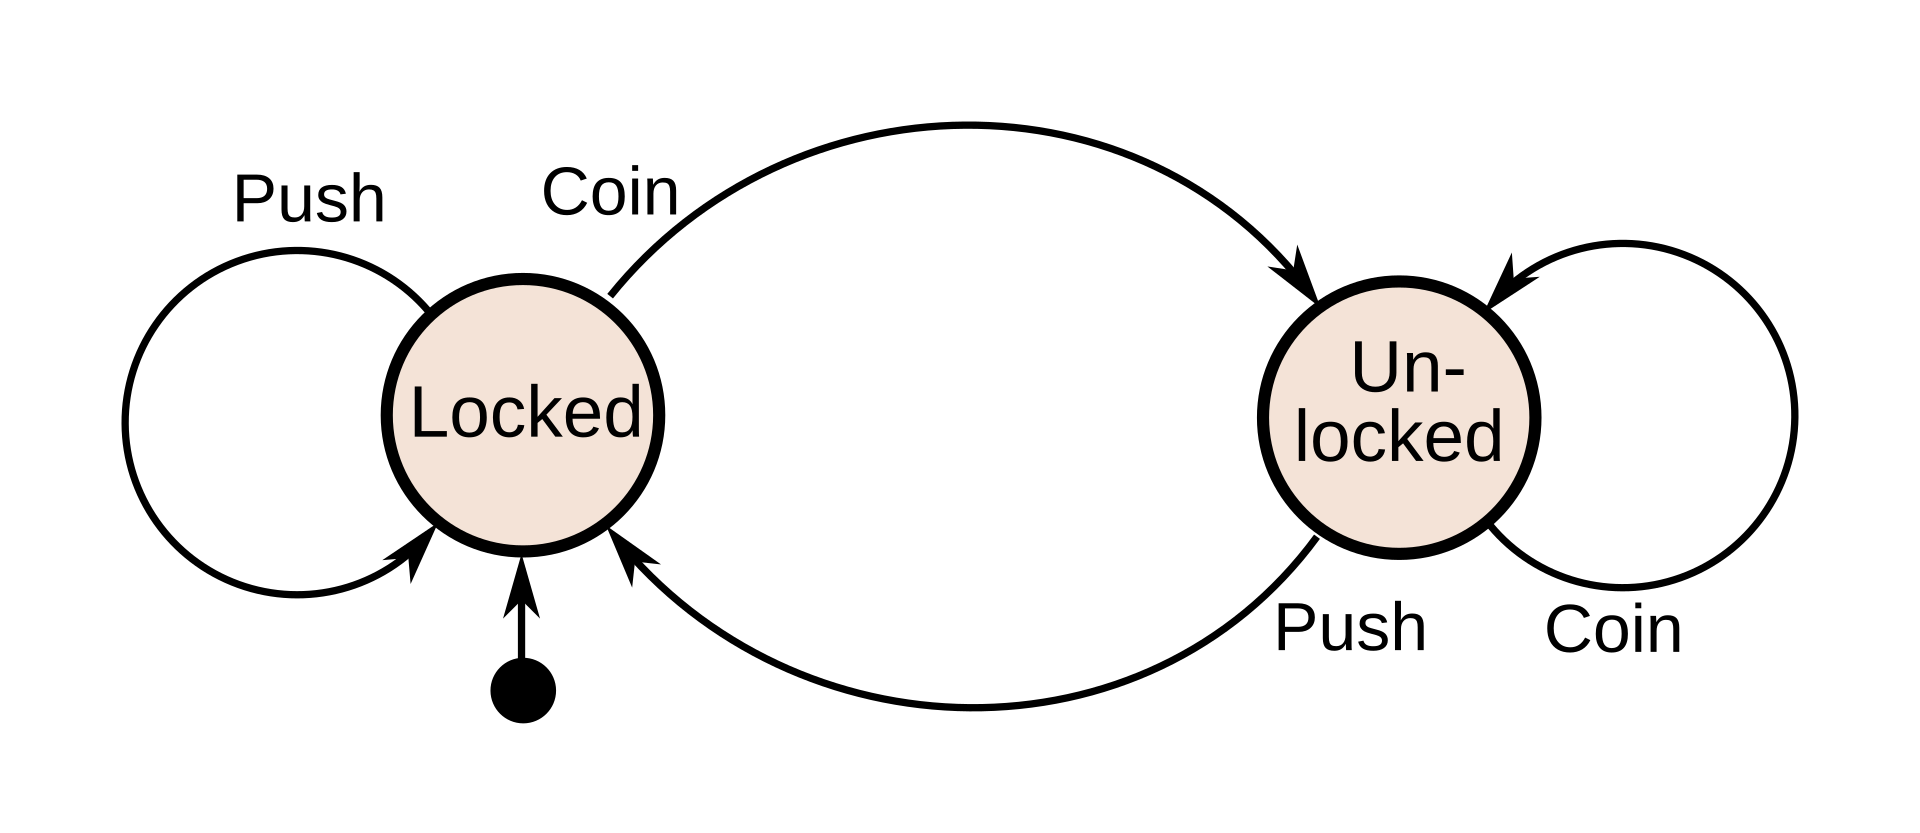
\includegraphics[width=0.7\textwidth]{img/fsm_turnstile.png}
    \caption{Turnstile FSM State Transition Diagram}
    \label{fig:fsm_turnstile_diagram}
\end{figure}

\begin{table}[H]
    \centering
    \begin{tabular}{|c|c|c|l|}
        \hline
        \textbf{Current State}    & \textbf{Input} & \textbf{Next State} & \textbf{Output}                                             \\
        \hline
        \multirow{2}{*}{Locked}   & Coin           & Unlocked            & Unlocks the turnstile so that the customer can push through \\
                                  & Push           & Locked              & None                                                        \\
        \hline
        \multirow{2}{*}{Unlocked} & Coin           & Unlocked            & None                                                        \\
                                  & Push           & Locked              & When the customer has pushed through, locks the turnstile   \\
        \hline
    \end{tabular}
    \caption{Turnstile FSM Transition Table}
    \label{tab:fsm_turnstile_table}
\end{table}

The FSM starts in the \textit{Locked} state.
When a coin is inserted, it transitions to the \textit{Unlocked} state and allows the customer to push through.
If the customer pushes through while in the \textit{Unlocked} state, the FSM transitions back to the \textit{Locked} state.
If a coin is inserted while in the \textit{Unlocked} state, the FSM remains in the same state.


\section{Parking Gate System}
\label{sec:parking_gate_system}

As already mentioned in the previous sections, the focus of this assignment is to model a parking gate system using finite state machines (FSMs).

\subsection{Requests}
\label{subsec:requests}

The requests that the parking gate system has to fullfil are the following:

\begin{itemize}
    \item Analyze the provided \textit{Vehicle FSM} and understand how it works;
    \item Define the \textit{raise} and \textit{lower} functions of the gate respecting $w_{max} = |4| [^\circ / s]$ and $\dot{w}_{max} = |1| [^\circ / s^2]$;
    \item Define the FSM to model the parking gate control system;
    \item Integrate the \textit{Vehicle FSM} and the parking gate control system FSM;
    \item Provide results of the simulation of the integrated system;
\end{itemize}

Notice that despite the suggestion from the professor to start from the already provided \textit{Vechicle FSM}, I decided to start from scratch in order to develop a deepened understanding of the FSMs, modelling also events, slightly more complex logics and composition / decomposition patterns.



\subsection{System Overview}
\label{subsec:system_overview}

The parking gate system is composed of two main components: the \textit{Vehicle FSM} and the \textit{Parking Gate FSM}.
The vehicle FSM is responsible for simulating the vehicle's behavior, while the parking gate FSM is responsible for controlling the gate's position and ensuring that it operates correctly in response to the vehicle's actions.

In Figure \ref{fig:parking_gate_system_overview} is shown the overview of the parking gate system.

\begin{figure}[H]
    \centering
    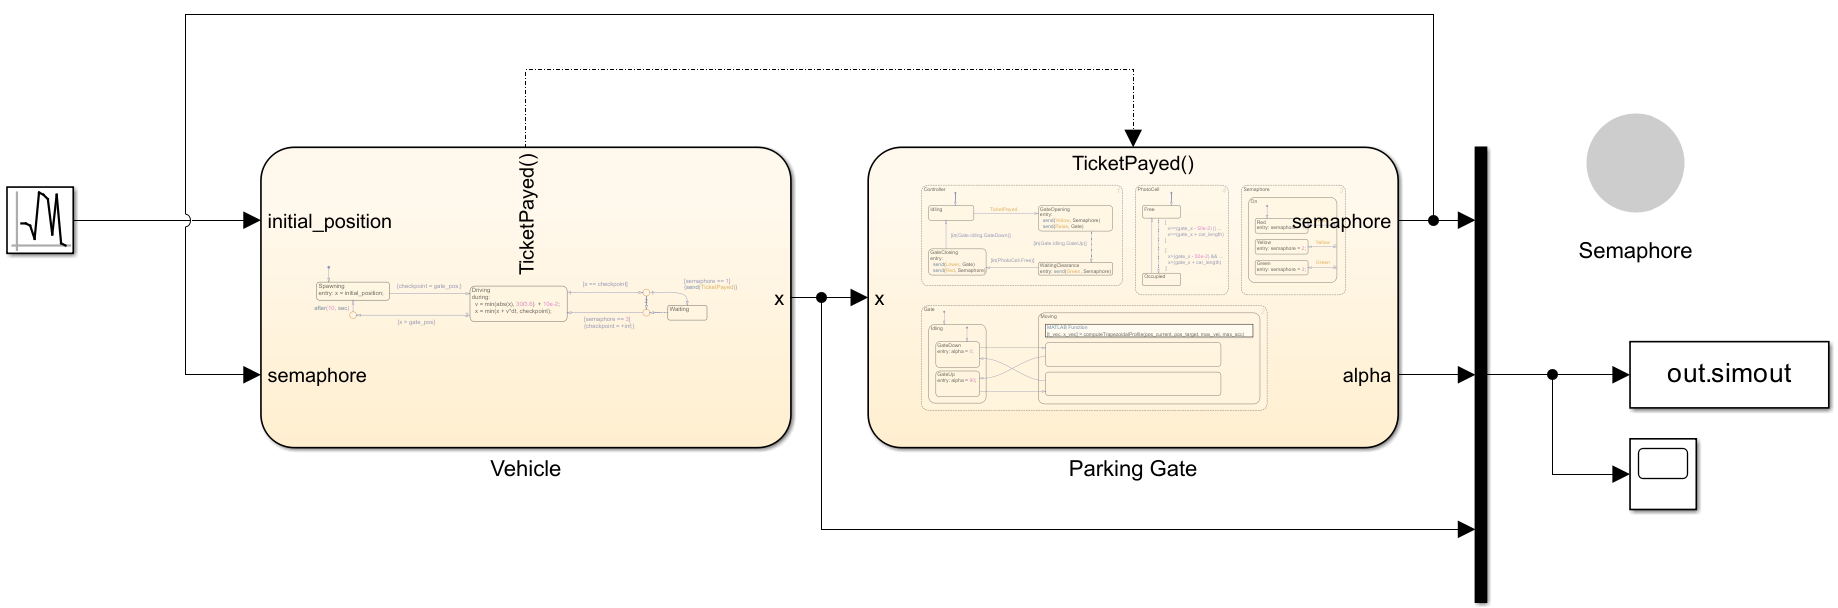
\includegraphics[width=1.0\textwidth]{./img/MATLAB/parking_gate_system_overview.png}
    \caption{Parking Gate System Overview}
    \label{fig:parking_gate_system_overview}
\end{figure}

It's already possible to understand which are the communication lines between the two FSMs:

\begin{itemize}
    \item The \textit{Vehicle FSM} sends the \textit{vehicle\_position (x)} to the \textit{Parking Gate FSM} to inform it about the vehicle's position in the parking lot;
    \item The \textit{Parking Gate FSM} sends the \textit{semaphore\_state} to the \textit{Vehicle FSM} to inform it about the state of the gate (closed, opening, opened);
    \item The \textit{Vehicle FSM} also sends the event about the \textit{ticket\_payment} to the \textit{Parking Gate FSM} to inform it that the vehicle has paid for the ticket and is ready to leave the parking lot;
\end{itemize}


\subsubsection{Vehicle FSM}
\label{subsubsec:vehicle_fsm}

The vehicle FSM is responsible for simulating the vehicle's behavior in the parking lot.
It has two main states: \textit{Driving} and \textit{Waiting}.
At first, the vehicle is initialized and given a random position ahead of the gate.
A checkpoint is also set so that it will stop at the gate before proceeding to the next state.
Once at the gate, the vehicle looks for the semaphore state: if the semaphore is green, it directly returns to the \textit{Driving} state and proceeds ahead to the next checkpoint which is now set to $+\infty$; instead, if the semaphore is red, it simulates the payment of the ticket by sending the event \textit{ticket\_payment} to the parking gate FSM and goes into the \textit{Waiting} state, waiting for the semaphore to turn green.
The vehicle proceed until the gate is closed again, when the external environment resets the vehicle to a new random position ahead of the gate to start the process again.

Figure \ref{fig:vehicle_fsm} shows the vehicle FSM.

\begin{figure}[H]
    \centering
    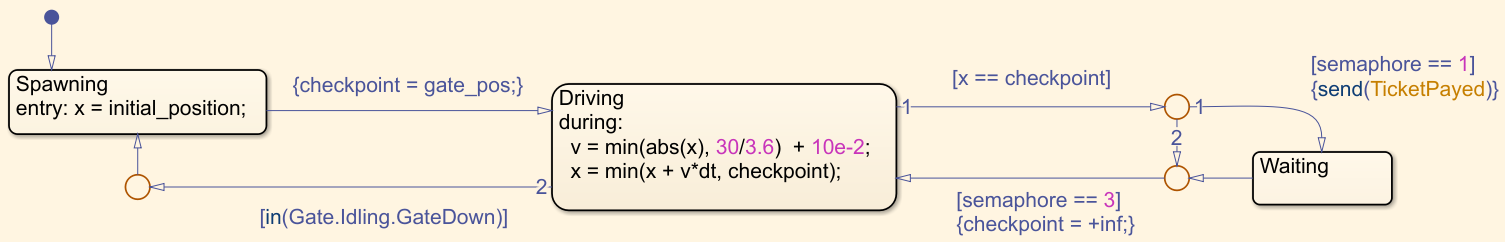
\includegraphics[width=1.0\textwidth]{./img/MATLAB/vehicle_fsm.png}
    \caption{Vehicle FSM}
    \label{fig:vehicle_fsm}
\end{figure}

Notice that the vehicle FSM has been modelled adopting the default \textit{OR} logic, meaning that the vehicle can assume only one state at a time (i.e. \textit{Driving} or \textit{Waiting}).



\subsubsection{Parking Gate FSM}
\label{subsubsec:parking_gate_fsm}

The parking gate FSM is responsible for controlling at first the gate's opening and closing, and then the semaphore state.
It has four main blocks: \textit{Controller}, \textit{Gate}, \textit{Semaphore} and \textit{PhotoCell}.


\paragraph{Controller}

The entry point of the parking gate FSM is the \textit{Controller} block, which is responsible for managing the overall state of the system and coordinating the other blocks.
It has been designed to be event-driven, meaning that communicates with the subcomponents of the system by sending and receiving events.
It has four main states: \textit{Idling}, \textit{GateOpening}, \textit{WaitingClearance} and \textit{GateClosing}.
At first, the \textit{Controller} block is in the \textit{Idling} state, waiting for the vehicle to arrive and send the \textit{ticket\_payment} event.
Once the ticket is paid, the \textit{Controller} block moves to the \textit{GateOpening} state, where it sends the \textit{RaiseGate} event to the \textit{Gate} block and the \textit{SemaphoreYellow} event to the \textit{Semaphore} block.
Once the gate is fully opened, the semaphore turns green and the \textit{Controller} block moves to the \textit{WaitingClearance} state, where it waits for the vehicle to pass through the gate.
Notice that the system determines the vehicle's position by using the \textit{PhotoCell} block, which is responsible for detecting the vehicle's presence in front of the gate.
Once the vehicle has passed through the gate, the \textit{Controller} block moves to the \textit{GateClosing} state, where it sends the \textit{LowerGate} event to the \textit{Gate} block and the \textit{SemaphoreRed} event to the \textit{Semaphore} block.
The \textit{Controller} block then moves back to the \textit{Idling} state, waiting for the next vehicle to arrive.

Figure \ref{fig:control_block} shows the \textit{Controller} block of the parking gate FSM.

\begin{figure}[H]
    \centering
    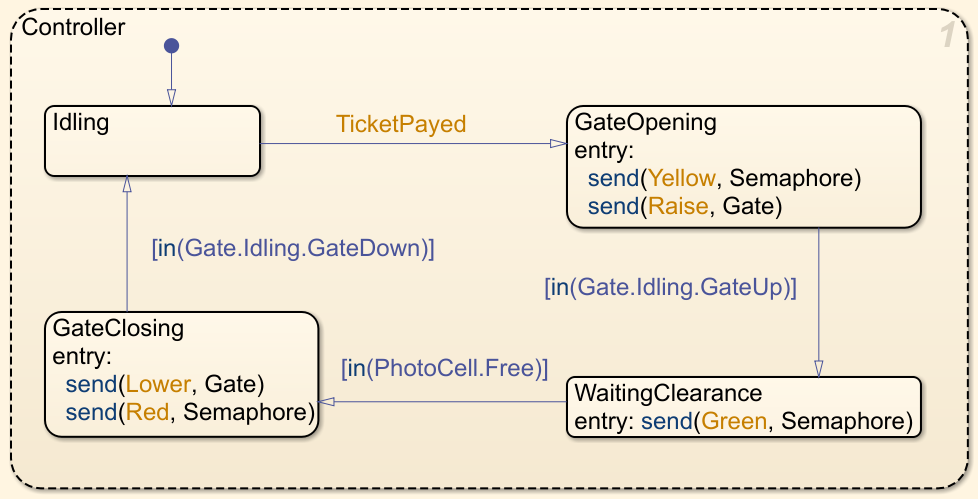
\includegraphics[width=0.8\textwidth]{./img/MATLAB/control_block.png}
    \caption{Control Block}
    \label{fig:control_block}
\end{figure}


\paragraph{Gate}

As already mentioned, the \textit{Gate} block is responsible for controlling the gate's position and ensuring that it opens and closes correctly.
It's designed based on two hierarchical states: \textit{Idling} and \textit{Moving}, which then are further divided into \textit{GateUp} and \textit{GateDown} states, and \textit{Raising} and \textit{Lowering} states, respectively.
At first, the \textit{Gate} block is in the \textit{GateDown} state, where the gate is closed and the vehicle is not allowed to pass through.
Once the \textit{RaiseGate} event is received from the \textit{Controller} block, the \textit{Gate} block moves to the \textit{Raising} state, where it starts to open the gate.
Once the gate is fully opened, the \textit{Gate} block moves to the \textit{GateUp} state waiting for the \textit{LowerGate} event from the \textit{Controller} block that will then perform the same steps in reverse order, moving to the \textit{Lowering} state and then to the \textit{GateDown} state once the gate is fully closed.

Figure \ref{fig:gate_block} shows the \textit{Gate} block of the parking gate FSM.

\begin{figure}[H]
    \centering
    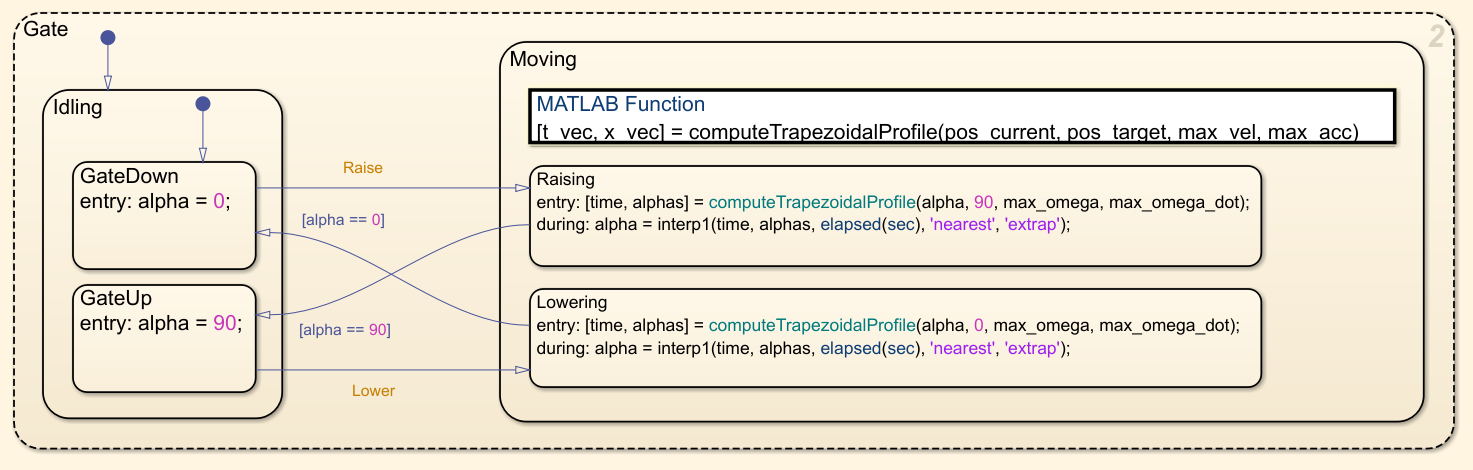
\includegraphics[width=1.0\textwidth]{./img/MATLAB/gate_block.png}
    \caption{Gate Block}
    \label{fig:gate_block}
\end{figure}

Notice that, in order to respect the constraints $w_{max} = |4| [^\circ / s]$ and $\dot{w}_{max} = |1| [^\circ / s^2]$, the position of the gate is updated based on the trapezoidal motion profile, generated when entering the \textit{Raising} or \textit{Lowering} states.
The trapezoidal motion profile is defined by the following equations:

\begin{equation}
    w(t) = \begin{cases}
        \frac{w_{max}}{t_1} t                   & t_0 \leq t < t_1 \\
        w_{max}                                 & t_1 \leq t < t_2 \\
        w_{max} - \frac{w_{max}}{t_3} (t - t_3) & t_2 \leq t < t_3
    \end{cases}
\end{equation}

Where $t_0$ is the time when the gate starts to open, $t_1$ is the time when the gate reaches the maximum speed and $t_2$ is the time when the gate starts to decelerate.
The trapezoidal motion profile is designed to ensure that the gate opens and closes smoothly, without any sudden jerks or stops.
Listing \ref{lst:trapezoidal_motion_profile} shows the implementation of the trapezoidal motion profile as MATLAB function.

\begin{lstlisting}[
    style=Matlab-editor,
    caption={Trapezoidal Motion Profile},
    label={lst:trapezoidal_motion_profile}
]
function [t_vec, x_vec] = computeTrapezoidalProfile(pos_current, pos_target, max_vel, max_acc)
% COMPUTE_TRAPEZOIDAL_PROFILE Generates time and angle points for a trapezoidal profile
% At first checks if a trapezoidal profile is feasible or is necessary to
% fallback to a triangular one.

delta_pos = pos_target - pos_current;
time_acc_phase = max_vel / max_acc;
delta_pos_acc_phase = 0.5 * max_acc * time_acc_phase^2;

if 2 * delta_pos_acc_phase < abs(delta_pos)
    % Trapezoidal profile
    t1 = time_acc_phase;
    t2 = (abs(delta_pos) - 2 * delta_pos_acc_phase) / max_vel;
    t3 = time_acc_phase;
else
    % Triangular profile
    max_vel = sqrt(abs(delta_pos) * max_acc);
    t1 = max_vel / max_acc;
    t2 = 0;
    t3 = max_vel / max_acc;
end


% Trapezoidal profile template (HP: s0 = 0, v0 = 0)
acc = max_acc * sign(delta_pos);
vel = max_vel * sign(delta_pos);
profile_template = @(t) ...
    (t <= t1) .*                             (1/2 * acc * t.^2) + ...
    (t > t1 & t <= (t1 + t2)) .*             (1/2 * acc * t1^2 + vel * (t - t1)) + ...
    (t > (t1 + t2) & t <= (t1 + t2 + t3)) .* (1/2 * acc * t1^2 + vel * t2 + vel * (t - (t2 + t1)) - 1/2 * acc * (t - (t1 + t2)).^2) + ...
    (t > (t1 + t2 + t3)) .*                  (1/2 * acc * t1^2 + vel * t2 + vel * t3 - 1/2 * acc * t3.^2);

% Profile generation
t_vec = linspace(0, t1 + t2 + t3, 100);
x_vec = profile_template(t_vec) + pos_current;

end
\end{lstlisting}


\paragraph{PhotoCell}

Despite being used only during the \textit{WaitingClearance} state of the \textit{Controller} block, the \textit{PhotoCell} block is responsible for detecting the vehicle's presence in front of the gate.
This, in fact, is the only way to understand if the vehicle has passed through the gate and the gate can be closed again.
In order to continuously sample the vehicle's position, the \textit{PhotoCell} block is designed to not be event-driven, but to move continuously between the two states \textit{VehiclePresent} and \textit{VehicleNotPresent} based on the vehicle's position.
By doing so, an external agent can continuously monitor the vehicle's position by checking the state of the \textit{PhotoCell} block.
In order to determines the presence or not of the vehicle, the \textit{PhotoCell} block uses the knowledge of the vehicle's position, which is sent by the \textit{Vehicle FSM} as an input to the \textit{Parking Gate FSM}.

Figure \ref{fig:photocell_block} shows the \textit{PhotoCell} block of the parking gate FSM.

\begin{figure}[H]
    \centering
    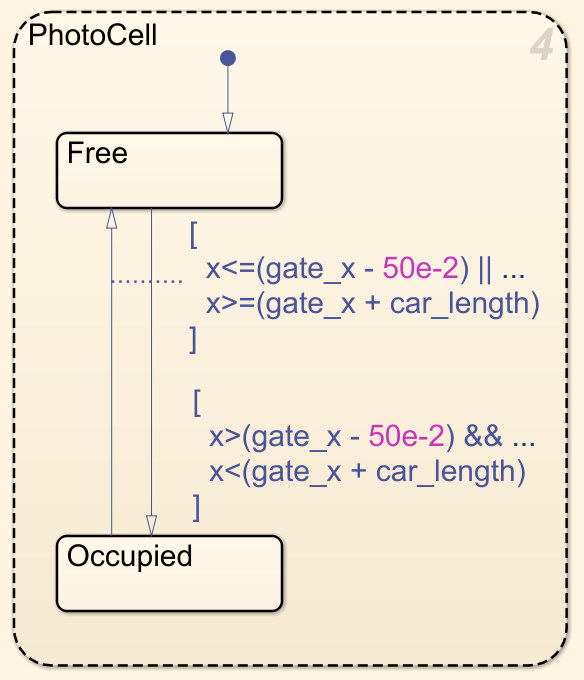
\includegraphics[width=0.4\textwidth]{./img/MATLAB/photocell_block.png}
    \caption{PhotoCell Block}
    \label{fig:photocell_block}
\end{figure}


\paragraph{Semaphore}

Last but not least, the \textit{Semaphore} block is responsible for switching the semaphore state between red, yellow and green based on the events received from the \textit{Controller} block.
It has one single state \textit{On} composed of  three sub-states representative of the color of the semaphore.
Based on the event received, the correct sub-state is chosen and the semaphore state is then sent to the \textit{Vehicle FSM} to inform it about the state of the gate (open, closed, etc.).
This is done in order to inform the vehicle about the state of the gate and allow it to proceed or stop based on the semaphore state, which is the only information that the vehicle has about the parking gate system (i.e. the vehicle doesn't know if the gate is open or closed, but only if the semaphore is red or green).

Figure \ref{fig:semaphore_block} shows the \textit{Semaphore} block of the parking gate FSM.

\begin{figure}[H]
    \centering
    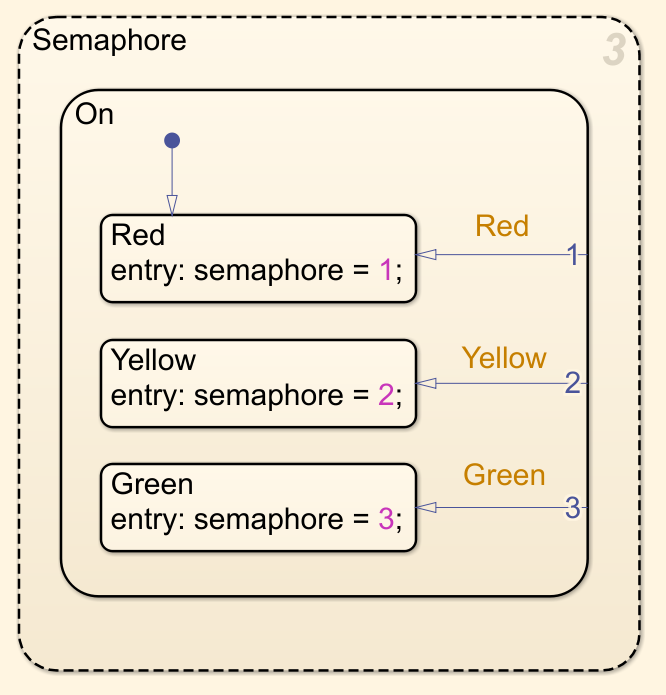
\includegraphics[width=0.5\textwidth]{./img/MATLAB/semaphore_block.png}
    \caption{Semaphore Block}
    \label{fig:semaphore_block}
\end{figure}



\subsection{Simulation Results}
\label{subsec:simulation_results}

The simulation has been run for $100s$ and the vehicle has been reset to a new random position after the gate has been closed.
The following figures show the results of the simulation.

\begin{figure}[H]
    \centering
    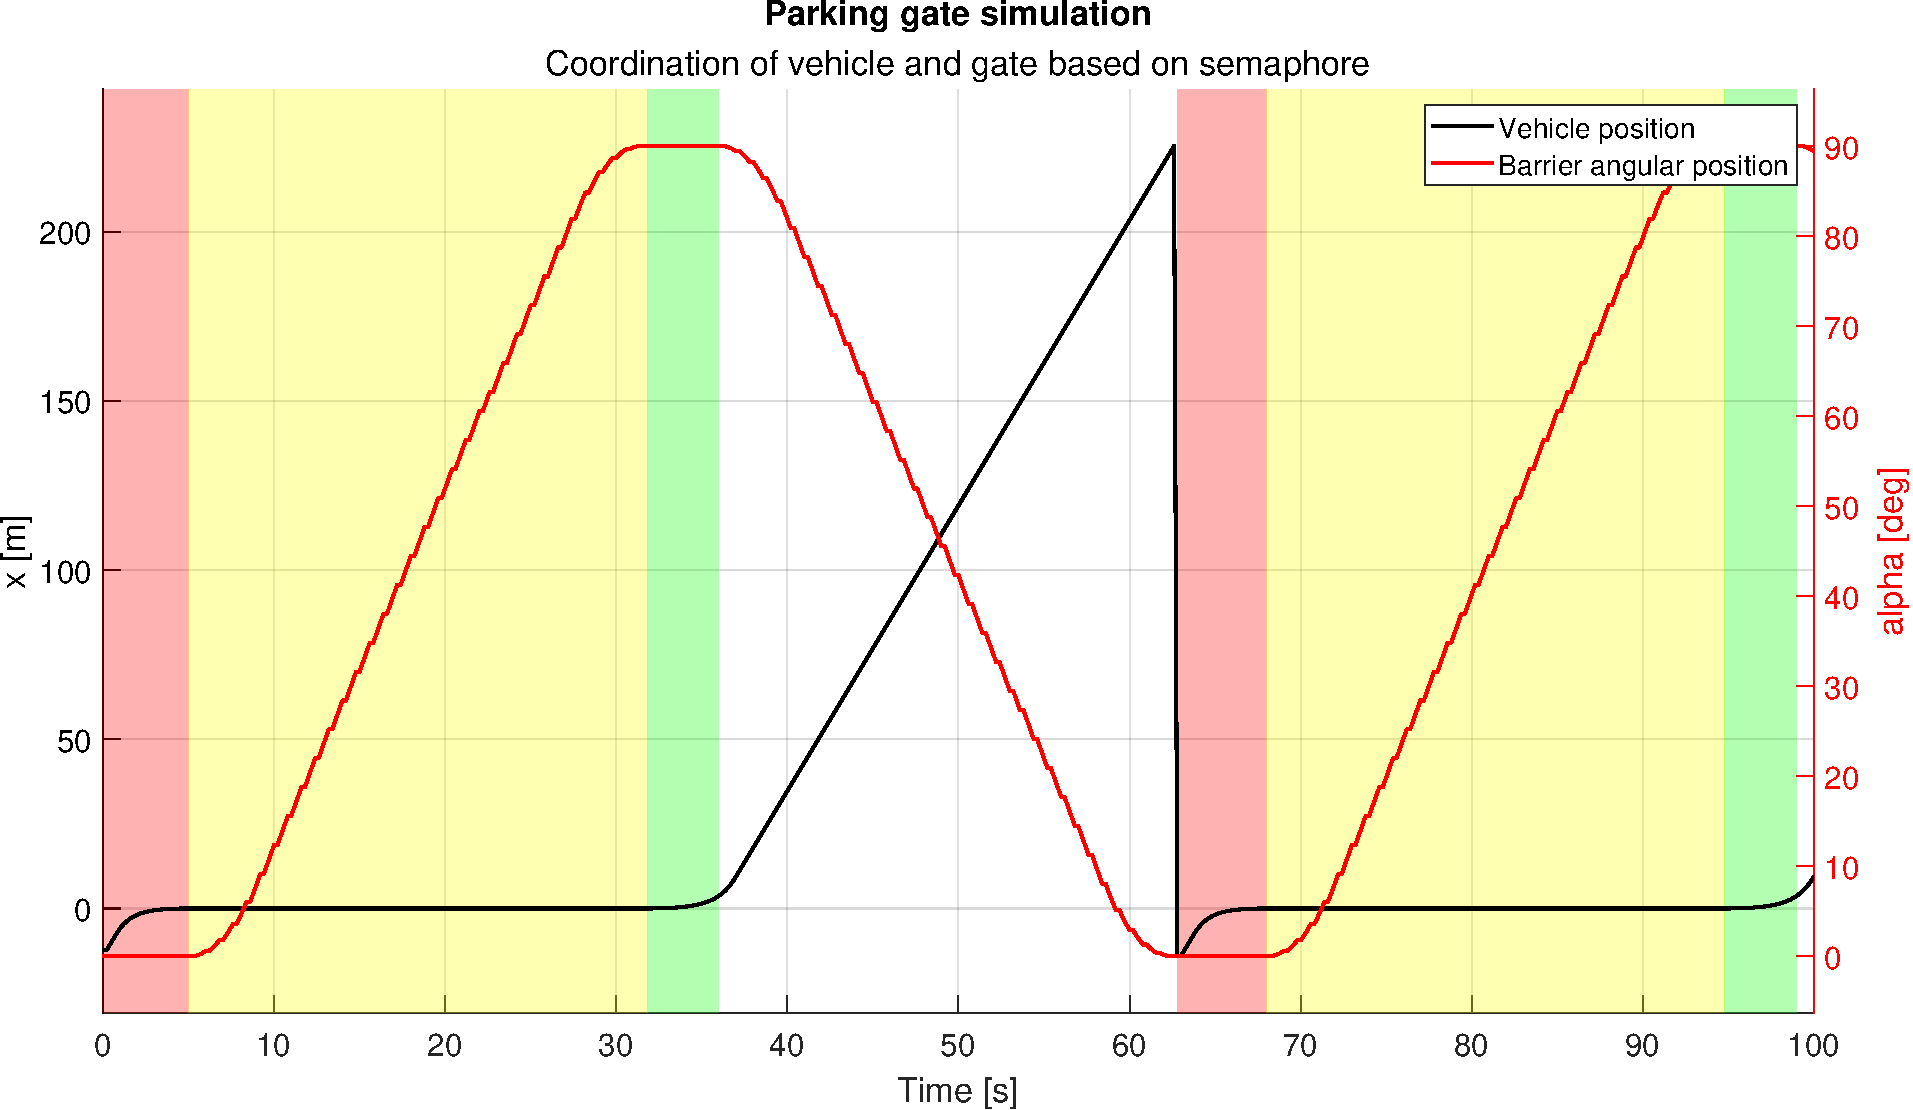
\includegraphics[width=1.0\textwidth]{./img/MATLAB/results.pdf}
    \caption{Simulation Results}
    \label{fig:simulation_results}
\end{figure}

Figure \ref{fig:simulation_results} shows the vehicle position (in black) and the gate position (in blue) over time.
The plot has also been divided into different regions based on the state of the \textit{Semaphore} block (red, yellow and green).
Notice that for clarity, the semaphore state has been added to the plot only when actually visible by the vehicle (i.e. when the vehicle is in front of the gate and not yet passed through it).

Instead, a more detailed view of the underlying coordination between the two FSMs is shown in Figure \ref{fig:simulation_results_detailed}, where a visualization of the state transitions and events is shown.
The plot report on the vertical axis the time of the simulation and on each vertical dashed line the state of each superstate of the FSMs is shown.
One can appreciate how the two FSMs are coordinated and how the events are sent and received between them, along with the transitions between the states.

\begin{figure}[H]
    \centering
    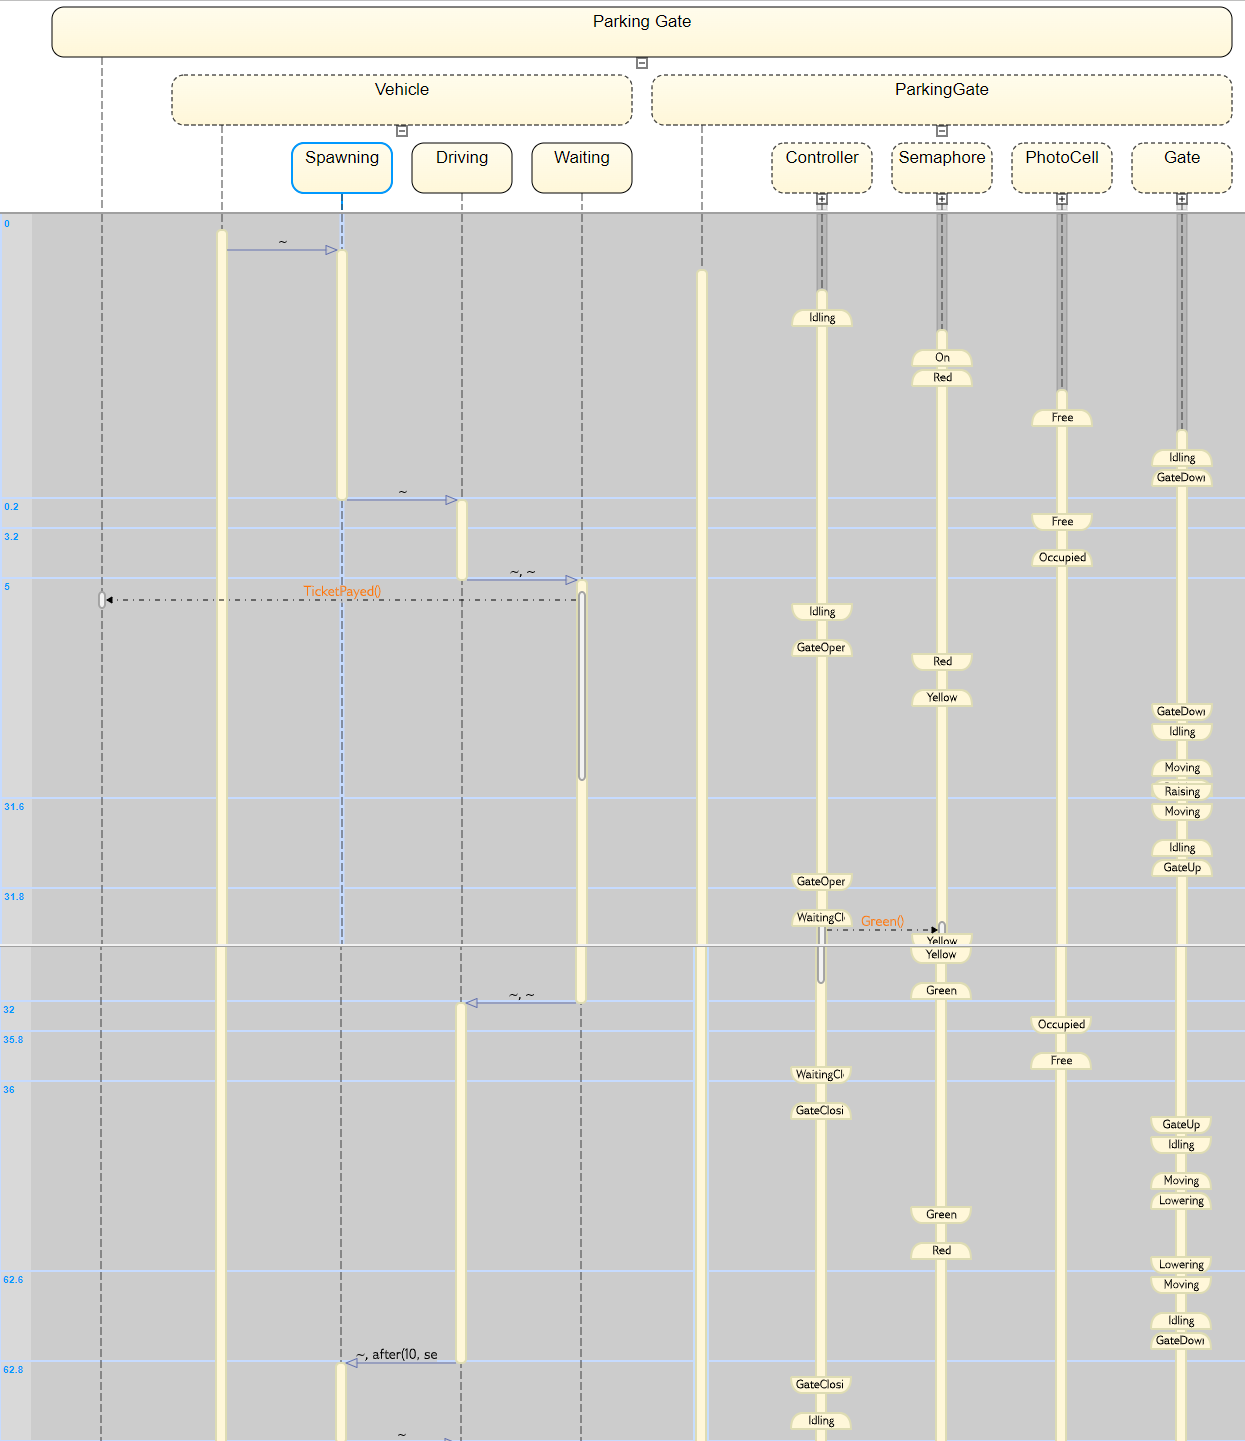
\includegraphics[width=1.0\textwidth]{./img/events.png}
    \caption{Simulation Results - Detailed View}
    \label{fig:simulation_results_detailed}
\end{figure}











\section{Conclusions}
\label{sec:conclusions}

In this short report, we have presented the results of the fifth assignment of the course on Autonomous Vehicles.
We have briefly explained what FSMs are and how they can be used to model the behavior of generic systems.

We have also presented a possible FMSs implementation about a car parking system, which is able to coordinate the behavior of the car and the parking gate.
The results presented have shown the effectiveness of the proposed solution.

The current solution could be improved under many aspects.
For example, one could think of implementing features like error handling, or ticket authentication and validation, or even a more complex parking system composed of multiple parking gates and cars that must coordinated over the network.

We believe that FMSs are a power tool that can often replace traditional programming paradigms, allowing to model complex systems in a more intuitive way.
Further studies on this topic could be useful to understand the full potential of FMSs and their applications in the field of autonomous vehicles and robotics in general.

\vspace*{\fill}
\nocite{*}
\bibliographystyle{plain}
\bibliography{references.bib}

\vspace*{\fill}
\appendix
\section{Appendix}

The system presented in Section \ref{subsec:system_overview}, leverages one single FSM including under the hood both the vehicle and the parking gate FSMs.
However, this solution is not the most elegant one given that the two FSMs are actually two separate entities that communicate with each other via external signals.
For this reason, the first solution and implementation of the parking gate system was the one shown in Figure \ref{fig:original_parking_gate_system_overview}.

\begin{figure}[H]
    \centering
    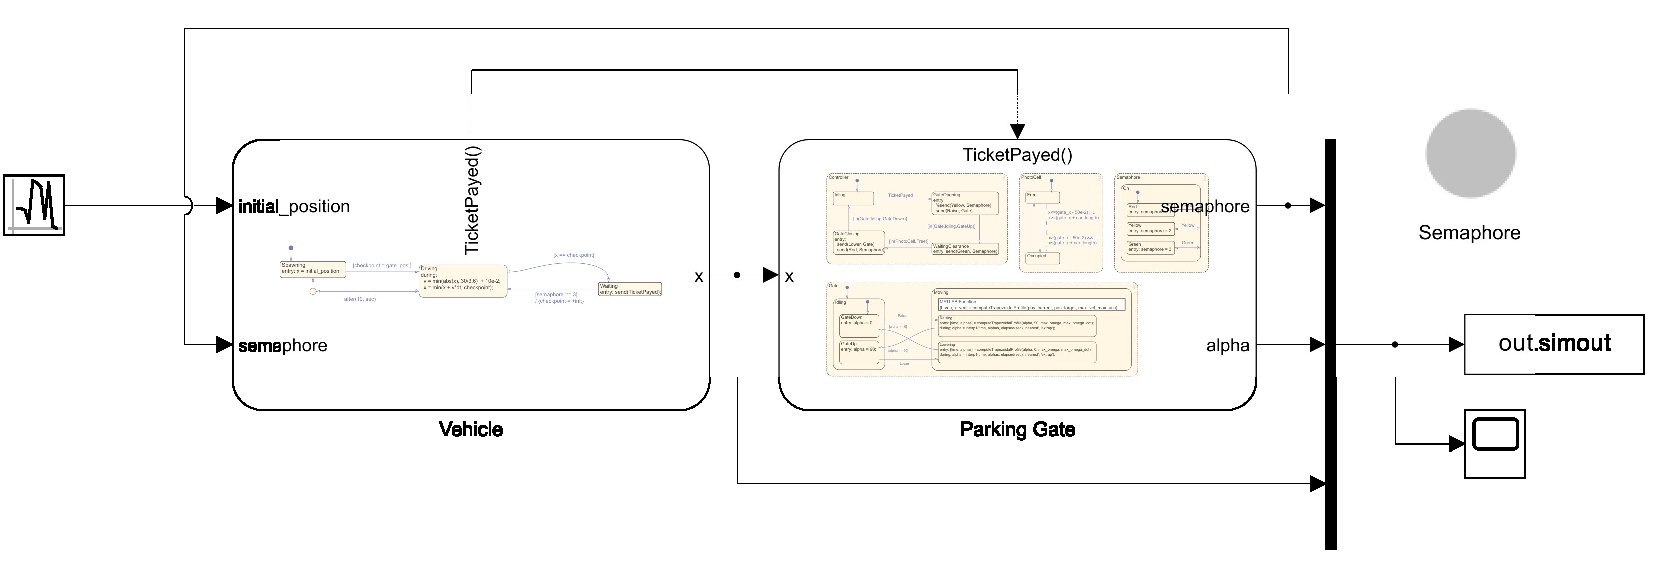
\includegraphics[width=1.0\textwidth]{./img/MATLAB/original_version.pdf}
    \caption{Original Parking Gate System Overview}
    \label{fig:original_parking_gate_system_overview}
\end{figure}

Notice that the underling components and states are exactly the same as the ones presented in the previous section.
Nonetheless, the structure of Figure \ref{fig:original_parking_gate_system_overview} resolved in unexpected behavior of the system and never generated the expected results.

Even with the help of debugging tools, it was impossible to understand the reason behind the unexpected behavior of the system and the author had to simplify the structure and fallback to the single FSM solution discussed during the document (compromise between elegance and functionality).

\end{document}
